\documentclass[a4paper,11pt]{article}

\usepackage{graphicx}  %%% for including graphics
\usepackage{url}       %%% for including URLs
\usepackage{times}
\usepackage{natbib}
\usepackage[margin=25mm]{geometry}
\usepackage{subcaption,graphicx}

\usepackage{tikz}
\tikzset{
    embedding/.style={rectangle,draw=black,text centered},
    index/.style={circle,draw=black,text centered, text width=0.45cm},
    hidden/.style={rectangle split,rectangle split horizontal=true,rectangle split parts=7,draw=black},
}
\usetikzlibrary{shapes,positioning,backgrounds}



\title{Multilingual Word Embeddings from Sentence Representations}
\date{}

%\author{Example Author\\
%       Affiliation\\
%       \texttt{example@email.org}
%  \and Someone Else\\
%       Another Affiliation\\
%       \texttt{another@email.org}
%}

\begin{document}
\maketitle
\thispagestyle{empty}
\pagestyle{empty}


\section*{Motivation}
%Why do we care about the problem and the results? If the problem isn't obviously "interesting" it might be better to put motivation first; but if your work is incremental progress on a problem that is widely recognized as important, then it is probably better to put the problem statement first to indicate which piece of the larger problem you are breaking off to work on. This section should include the importance of your work, the difficulty of the area, and the impact it might have if successful.



% Practical: multilingual IR
% Theoretical: multilinguality (arguably) results in better conceptual space
Distributional semantics concerns the establishment of a semantic space where words are represented by vectors and their relations have a geometrical interpretation. We investigated how to use data from multiple languages to create a single semantic space. In particular, we induce word embeddings for seven languages in a shared space.  

This allows for linguistic inquiry into semantic differences between vocabularies. The latent conceptual semantic space can arguably be approximated more closely by using multilingual data, as language-specific effects fade away. 
Moreover, a joint semantics space of many languages allows for tasks such as multilingual Information Retrieval without using a pivot language.


%, and structured prediction tasks like Machine Translation. Moreover, this allows for linguistic inquiry into semantic differences between vocabularies. The latent conceptual semantic space can arguably be approximated more closely by using multilingual data, as language-specific effects fade away. %We show that we can actually improve performance on monolingual tasks. 
%However, syntactic features of word embeddings partly depend on the language and may thus suffer from this approach.

% lots of languages together is cool
%In particular, we induce word embeddings for seven languages in a shared space.  This allows for linguistic inquiry into semantic differences between vocabularies. It is also useful for tasks in which relevant resources might exist in many languages, %such as question answering, sentiment analysis and information retrieval, 
%or tasks in which we would like to compare resources across languages%, e.g. to compare international differences in attitude
%.

% multilingual training is also good for monolingual semantics
%The multi-lingual training signal can also improve performance on monolingual tasks. Incorporating information across languages leads to a richer semantic space, that might be less prone to language-specific capriciousness. While this smoothness is most useful in a complex model that also accounts for word senses and composition, we show that this smoothness is already useful in a simple model. %SMOOTHNES??
% dit stuk is een beetje dubbelop



%Practical: multilingual IR
%Theoretical: multilinguality (arguably) results in better conceptual space

%Distributional semantics is a fast developing field that concerns the establishment of a semantic vector space were words have a geometrical interpretation. We investigated how to use data in multiple languages to create a single multilingual semantic space. The word representations in this vector space may have a theoretical interest on their own right, but can also be used for tasks related to translation, such as cross-lingual information retrieval and machine translation. 





\section*{Problem statement and related work}
%What problem are you trying to solve? What is the scope of your work (a generalized approach, or for a specific situation)? Be careful not to use too much jargon. In some cases it is appropriate to put the problem statement before the motivation, but usually this only works if most readers already understand why the problem is important.



We want to induce a multilingual semantic space, in which words that are translations of each other are close together. 
\cite{klementiev2012inducing} propose a multi task learning formulation of this problem. An interaction-matrix expressing the relatedness of words in both languages is defined, based on word alignments. When a word is trained, other words are co-trained depending on their interaction score.

However, we aim to fulfill the task without using word alignments, just from parallel data. Word embeddings can be based on either local or global co-occurrence. The former relies on a context of words before or around the target word. However, without word alignments there is no apparent way to define the same context window in parallel sentences. Therefore we rely on global co-occurrence: the fact that words occur in the same sentence. 

%Global co-occurrence information does not provide information about the syntactic and semantic role a word plays in a sentence, but moreover expresses topicality. We thus expect the resulting word-embeddings to be useful for IR-related tasks rather than structured predictions.

\cite{hermann2014multilingual} also approach the task without using word alignments. They rely on a model of composition which can range from a simple bag-of-words additive model to a syntactically motivated model. The word embeddings and the compositional model determine the representation of a sentence. The learning objective is to minimize the distance between the representations of parallel sentences, by backpropagating the error to the word embeddings.
The work of \cite{sarath2014autoencoder} treats the multilingual sentence representation as a hidden layer in an auto-encoder. Word representations are learned by reconstructing which words occur in both aligned sentences. 


% waar zou dit stuk moeten?
%We induce word embeddings using a distributional representation of the bitext sentence. In this respect, our work is related to \cite{hermann2014multilingual} and \cite{SarathChandar2014autoencoder}. The work of \cite{hermann2014multilingual} proposes a general method for inducing word representations by minimizing the distance between representations of aligned sentences in contrast to unaligned sentences, and backpropagating the error signal to the word embeddings. The work of \cite{SarathChandar2014autoencoder} treats the multilingual sentence representation as a hidden layer in an auto-encoder, and learns word representations by reconstructing which words occur in both aligned sentences. Both of these methods do not rely on word alignments, and extract word embeddings from a distributional representation of the sentence. We do this directly from a simple and efficient model of sentence representations. % niet-helemaal-lekkere-zin



\section*{Approach}
%How did you go about solving or making progress on the problem? Did you use simulation, analytic models, prototype construction, or analysis of field data for an actual product? What was the extent of your work (did you look at one application program or a hundred programs in twenty different programming languages?) What important variables did you control, ignore, or measure?


We also extract word embeddings from a distributional representation of the sentence. However, we rely on a very simple and efficient model of sentence representations without requiring an explicit compositional model. 
%Instead of backpropagating an error to word embeddings in a network, we use a simple definition of word embeddings. 
%We do not backpropagate an error to word embeddings, but simply define words as the average of the sentences they occur in.

%Extended Paragraph2vec \cite{Le2014} for multilingual case

\cite{le2014distributed} introduce {\tt paragraph2vec}, a model to obtain embeddings for paragraphs, i.e. sequences of words that may range from phrases  to entire documents. The {\tt PV-DBOW} version of the model predicts the indexes of all words that occur in a sentence with a hierarchical softmax layer, thus viewing the paragraph as a bag-of-words. 

We extend this model to the multilingual case, which is depicted in figure~\ref{f:model}, where $w_n^{l_x}$ is the $n$th word in the sentence~$x$ in language~$l$. A single sentence representation is instantiated for parallel sentences, from which the network predicts words that occur in the sentence in either language. This extension can easily be applied to more than 2 languages.%: in principle, sentences in any number of languages can be trained as long as they are parallel across all languages.

\begin{figure}\center
\begin{subfigure}{.49\linewidth}
\center
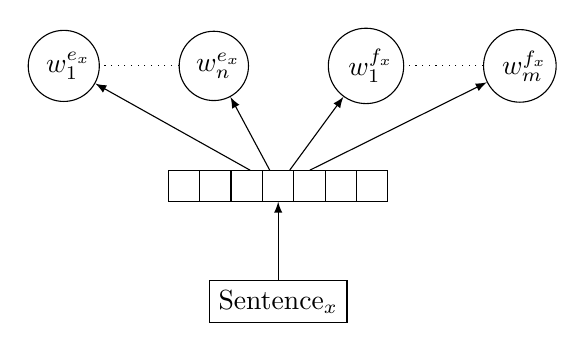
\begin{tikzpicture}[>=latex] 
\node[embedding] (Sx) {Sentence$_x$};
\node[hidden] (h1)[above=of Sx]{} edge [<-] (Sx);
\node[index] (We1) [above left =of h1] {$w^{e_x}_1$} edge [<-] (h1);
\node[index] (Wen) [right =of We1] {$w^{e_x}_n$}edge [<-] (h1) edge [ dotted ] (We1);
\node[index] (Wf1) [right =of Wen] {$w^{f_x}_1$}edge [<-] (h1) ;
\node[index] (Wfm) [right =of Wf1] {$w^{f_x}_m$}edge [<-] (h1) edge [ dotted ] (Wf1);
\end{tikzpicture}
\caption{Extension of {\tt PV-DBOW} for parallel sentences.}
\label{f:model}
\end{subfigure}
\begin{subfigure}{.49\linewidth}
\flushright
\begin{tabular}{c | r r r r }
&	\multicolumn{4}{c}{Classification [train]-[test]}	\\
&EN-EN	&DE-DE	&DE-EN	&EN-DE		\\\hline
EN			&.274		&.286		&.305		&.284		\\
DE			&.263		&.190		&.166		&.270		\\
DE-EN			&.319		&.304		&.264		&.323		\\
\end{tabular}
\caption{F1 scores on TED classification task for sentence representations and word representations. The left column denotes the training data	for	the word embeddings. }
\label{t:dbow_mono_bi}
\end{subfigure}
\caption{Model and results}
\end{figure}


%Word embeddings as sentence average
Word embeddings are defined to be the average of all sentences they occur in. This is  formalized in equation~\ref{e:words}, where $[\![ x ]\!]$ denotes the (distributional) representation of $x$, $freq(w,x)$ is the frequency of word $w$ in $x$, and $s\in D$ are sentences $s$ in the training data $D$.
\begin{equation}
[\![ w ]\!] =\frac{1}{freq(w,D)}\sum_{s\in D}freq(w,s) [\![ s ]\!]
\label{e:words}
\end{equation}

We thus obtained word embeddings from either 500 k sentences of aligned Europarl data in English-German, or 50 k sentences aligned between seven languages. We used English as a pivot language to cross-lingually align those sentences.

%The data in all languages is originally paired with English, which we used as a pivot language for the cross-lingual alignment of sentences.

%Evaluation: analogy and crosslingual document classification
%Evaluation of cross-lingual word embeddings is not trivial. We apply a word analogy task to measure the quality of the English word embeddings. 
To evaluate the inter-lingual consistency, we run the cross-lingual document classification task introduced by~\cite{klementiev2012inducing} with two different datasets. In this task, a document classifier is trained using word embeddings in one language, and tested on word embeddings in another language. 


\section*{Results}
%What's the answer? Specifically, most good computer architecture papers conclude that something is so many percent faster, cheaper, smaller, or otherwise better than something else. Put the result there, in numbers. Avoid vague, hand-waving results such as "very", "small", or "significant." If you must be vague, you are only given license to do so when you can talk about orders-of-magnitude improvement. There is a tension here in that you should not provide numbers that can be easily misinterpreted, but on the other hand you don't have room for all the caveats.
Using embeddings from multilingually trained sentence representations improves performance on the cross-lingual document classification tasks, as illustrated for the bilingual case in table~\ref{t:dbow_mono_bi}. This effect may partially be explained by there being more training data: two versions of each sentence are used to train the sentence embeddings. 

However, we also see the that word embeddings trained on English data only are more useful for the classification even of German documents, possibly because of the richer German morphology and larger vocabulary. This indicates that useful information from one language can be transferred to another by means of the shared semantic space.





%Classification improves from parawords, even transfer to other language!




\section*{Conclusions}
%What are the implications of your answer? Is it going to change the world (unlikely), be a significant "win", be a nice hack, or simply serve as a road sign indicating that this path is a waste of time (all of the previous results are useful). Are your results general, potentially generalizable, or specific to a particular case?


We came up with a simple model to obtain cross-lingual sentence embeddings in any number of languages, that is easy and cheap to train. Word embeddings are determined in a straightforward fashion. Information from one language can increase performance on document classification in another language. 


%Set-up can be generalized to complex compositionality, e.g. syntactic parser for one language and not for other?

%Relation to other models?







%\section{Introduction}
%....

\bibliographystyle{chicago}
\bibliography{bibliography}

\end{document}

%\begin{abstract}
%
%By representing the meaning of language in a vector space, we can model many semantic phenomena in a natural way.
%These representations have also proven useful for many Natural Language Processing tasks.
%We propose a method for using multilingual sentence embeddings to construct word embeddings in a shared vector space.
%We also highlight the difference between approaches that rely on local word context and on co-occurrence within sentences.
%Our model learns word embeddings that share features across multiple languages.
%We evaluate our word embeddings on a cross-lingual document classification task on two corpora.
%
%
%\end{abstract}
